\documentclass[11pt, oneside]{article} 
\usepackage{geometry}
\geometry{letterpaper} 
\usepackage{graphicx}
	
\usepackage{amssymb}
\usepackage{amsmath}
\usepackage{parskip}
\usepackage{color}
\usepackage{hyperref}

\graphicspath{{/Users/telliott_admin/Dropbox/Tex/png/}}
% \begin{center} 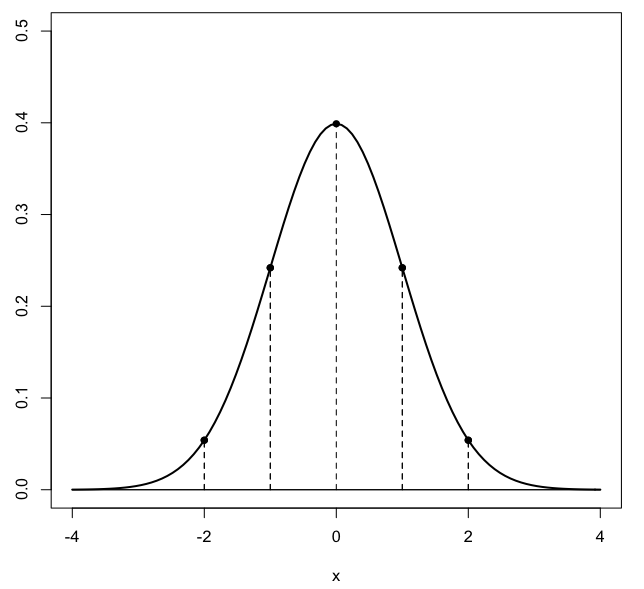
\includegraphics [scale=0.4] {gauss3.png} \end{center}

\title{Continued fractions}
\date{}

\begin{document}
\maketitle
\Large
Continued fractions are awkward, but they're powerful.

\url{http://www.mathpath.org/concepts/cont.frac.htm}

\subsection*{rational number}
Consider $153/53$
\[ \frac{153}{53} = 2 + \frac{47}{53} = 2 + \frac{1}{53/47} \]
But
\[ \frac{53}{47} = 1 + \frac{6}{47} = 1 + \frac{1}{47/6}  \]
And
\[ \frac{47}{6} = 7 + \frac{5}{6} = 7 + \frac{1}{6/5}  \] 
And
\[ \frac{6}{5} = 1 + \frac{1}{5} \] 
All together
\[ \frac{153}{53} = 2 + \cfrac{1}{1 + \cfrac{1}{7 + \cfrac{1}{1 + \cfrac{1}{5}}}} \]
Hard to think about, and hard to write, let alone typeset.  

If all the numerators are $1$'s like this, the continued fraction is called simple.

Really, this is just the Euclidean algorithm in disguise.  And that algorithm must terminate, for a \emph{rational} (fractional) number.

One alternative representation is
\[ 2 + \frac{1}{1+} \ \frac{1}{7+} \ \frac{1}{1+} \ \frac{1}{5} \]

The continued fraction representation may also be written as
\begin{verbatim}
153/53 = [2,1,7,1,5]
\end{verbatim}

To go backwards:
\begin{verbatim}
1 + 1/5 = 6/5
7 + 5/6 = 47/6
1 + 6/47 = 53/47
2 + 47/53 = 153/53
\end{verbatim}

\subsection*{square root of 2}
One can also find continued fraction representations of irrational numbers like $\sqrt{2}$.  However, since the difference is that these cannot terminate (because they are not rational, i.e. fractional).

\[ (\sqrt{2} - 1)(\sqrt{2} + 1) = 1 \]
Rearrange to get a substitution we will use again
\[ \sqrt{2} - 1 = \frac{1}{\sqrt{2} + 1} \]

At the same time, add one and subtract one on the bottom right:
\[ \sqrt{2} - 1 =  \frac{1}{2 + \sqrt{2} - 1} \]
substitute
\[ = \frac{1}{2 + \frac{1}{\sqrt{2} + 1}} \]
Add one and subtract one again and then substitute
\[ = \frac{1}{2 + \frac{1}{2 + \sqrt{2} - 1}} = \frac{1}{2 + \frac{1}{2 + \frac{1}{\sqrt{2} + 1} }} \]
Clearly, this goes on forever.
\[ \sqrt{2} = 1 + \cfrac{1}{2+\cfrac{1}{2+\cfrac{1}{2 + \dots}}}  \]

The continued fraction representation of $\sqrt{2}$ is $[1:2]$, meaning that there is an initial $1$ followed by repeated $2$'s.

To turn this into an approximate decimal representation of $\sqrt{2}$, ignore the $\dots$.  Then the last fraction is $5/2$.  Invert and add, repeatedly:

\begin{verbatim}
2 + 1/2 = 5/2
2 + 2/5 = 12/5
2 + 5/12 = 29/12
2 + 12/29 = 71/29
2 + 29/71 = 171/71
2 + 71/171 = 413/171
\end{verbatim}

To terminate:
\begin{verbatim}
1 + 171/413 = 584/413 = 1.414043
\end{verbatim}

To six places, $\sqrt{2} = 1.414213$.  We have three.

\subsection*{square root of 3}
The continued fraction representation of $\sqrt{3}$ is $[1,1,2,1,2, \dots]$.

This can be shortened to $[1:(1,2)]$.  Here is a derivation:

\[ (\sqrt{3} - 1)(\sqrt{3} + 1) = 2 \]
\[ \sqrt{3} - 1 = \frac{2}{\sqrt{3} + 1}   \]
\[ \frac{\sqrt{3} - 1}{2} = \frac{1}{\sqrt{3} + 1} \]
both of which we will use again.  However, going further, add and subtract on the bottom right
\[ \sqrt{3} - 1 = \frac{2}{\sqrt{3} + 1}  = \frac{2}{2 + \sqrt{3} - 1} \]
Divide top and bottom by $2$
\[ = \frac{1}{1 + \frac{\sqrt{3} - 1}{2}} \]
and substitute giving
\[= \frac{1}{1 + \frac{1}{\sqrt{3} +1}} \]
That's the end of step 1.

Now, for the second step, we focus on that last fraction
\[ \frac{1}{\sqrt{3} +1} = \frac{1}{2 + \sqrt{3} -1} = \frac{1}{2 + \frac{2}{\sqrt{3} + 1}} \]

Then for step three, we focus again on the last fraction, which is what we worked with in the first part.
\[ \frac{2}{\sqrt{3} + 1} = \frac{1}{1 + \frac{1}{\sqrt{3} +1}} \]

So now both terms repeat:
\[ \sqrt{3} - 1 = \cfrac{1}{1+\cfrac{1}{2+\cfrac{1}{1 + \cfrac{1}{2 + \dots }}}}  \]

which is $[1:(1,2)]$, as we said.

We can get approximations for $\sqrt{3}$ similar to what we did for $\sqrt{2}$.  Unlike previously, here there are two possibilities.  We start with either one of
\[ 1 + \frac{1}{2 + \dots} \]
\[ 2 + \frac{1}{1 + \dots} \]
and start by ignoring the dots.

The first gives
\begin{verbatim}
1 + 1/2 = 3/2
2 + 2/3 = 8/3
1 + 3/8 = 11/8
2 + 8/11 = 30/11
1 + 11/30 = 41/30
2 + 30/41 = 112/41
1 + 41/112 = 153/112

1 + 112/153 = 265/153 = 1.732026
\end{verbatim}

The actual value is $\sqrt{3} = 1.732051$, to six places.  We have four.

The second gives
\begin{verbatim}
2 + 1 = 3
1 + 1/3 = 4/3
2 + 3/4 = 11/4
1 + 4/11 = 15/11
2 + 11/15 = 41/15
1 + 15/41 = 56/41
2 + 41/56 = 153/56
1 + 56/153 = 209/153
2 + 153/209 = 571/209
1 + 209/571 = 780/571

1 + 571/780 = 1351/780 = 1.732051
\end{verbatim}

The actual value is $\sqrt{3} = 1.732051$, to six places.  We have all six.

\end{document}
